

\begin{figure}[ht] % https://www.math.u-bordeaux.fr/gtem2008/TikZ/main.pdf
    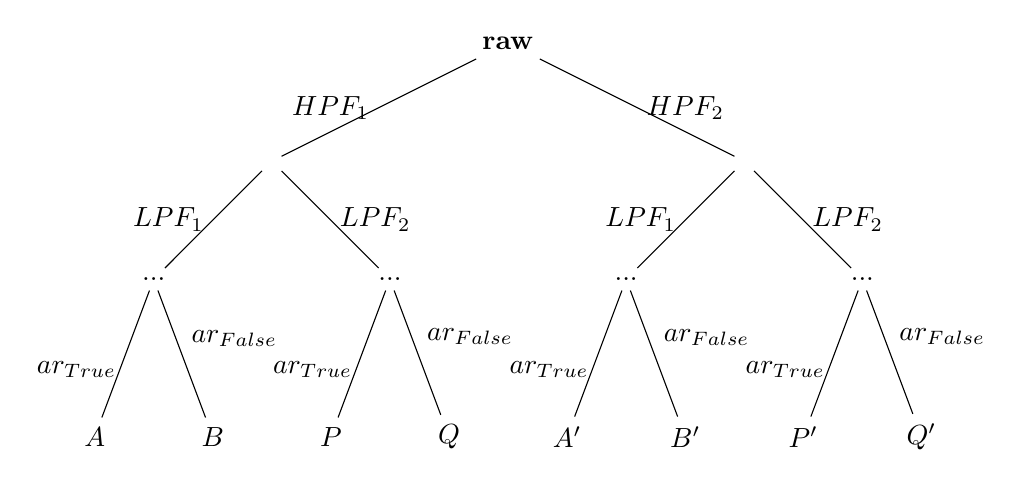
\begin{tikzpicture} 
    \tikzset{
        level 1/.style={level distance=15mm, sibling distance=60mm},
        level 2/.style={level distance=15mm, sibling distance=30mm},
        level 3/.style={level distance=20mm, sibling distance=15mm}
    }
    \node {\textbf{raw}}
        child {node { } 
            child {node { ... }
                child {node {$A$} edge from parent node[left, yshift=-2mm] {$ar_{True}$}}
                child {node {$B$} edge from parent node[right, yshift=2mm] {$ar_{False}$}}
                edge from parent node[left] {$LPF_1$}}
            child {node { ... } 
                child {node {$P$} edge from parent node[left, yshift=-2mm] {$ar_{True}$}}
                child {node {$Q$} edge from parent node[right, yshift=2mm] {$ar_{False}$}}
                edge from parent node[right] {$LPF_2$}}
            edge from parent node[left, yshift=0mm] {$HPF_1$}
        } 
        child {node { } 
            child {node { ... }
                child {node {$A'$} edge from parent node[left, yshift=-2mm] {$ar_{True}$}}
                child {node {$B'$} edge from parent node[right, yshift=2mm] {$ar_{False}$}}
                edge from parent node[left] {$LPF_1$}}
            child {node { ... } 
                child {node {$P'$} edge from parent node[left, yshift=-2mm] {$ar_{True}$}}
                child {node {$Q'$} edge from parent node[right, yshift=2mm] {$ar_{False}$}}
                edge from parent node[right] {$LPF_2$}
            }
            edge from parent node[right, yshift=0mm] {$HPF_2$}
        };
    
    \end{tikzpicture}

    \caption{\color{Gray} \textbf{Simplified excerpt from the multiverse}. Processing decisions are made at each hierarchical level, resulting in multiple different datasets (children). For evaluating the impact of some processing step (e.g., using $HPF_1$)  to its alternative (e.g., $HPF_2$), one could compare the respective leaf nodes to each other ($A$ with $A'$, $B$ with $B'$, and so forth). Those respective leaf nodes only differed in the choice of $HPF$ but were similar in all other processing steps. Similarly, one could average over some outcome metric of each of raw's children individually for each participant for comparison. Ellipses at level 2 indicate the presence of more levels, which alongside with the respective branches and leaf nodes were not visualized for brevity. }     
    \label{fig_tree}
    
\end{figure}
